\documentclass[11pt]{article}
% Shared preamble for the notes in this repository. pdfLaTeX, TeX Live 2024 or later.
\usepackage[a4paper,margin=2.6cm]{geometry}
\usepackage[T1]{fontenc}
\usepackage{lmodern}
\usepackage{microtype}
\usepackage{amsmath,amssymb,amsthm}
\usepackage{graphicx}
\usepackage{booktabs}
\usepackage{enumitem}
\usepackage[dvipsnames]{xcolor}
\usepackage[hidelinks]{hyperref}
\hypersetup{colorlinks=true,linkcolor=MidnightBlue,citecolor=MidnightBlue,urlcolor=MidnightBlue}
\graphicspath{{../../figures/}}
\setlist{itemsep=2pt,topsep=4pt}

\newtheorem{theorem}{Theorem}
\newtheorem{proposition}[theorem]{Proposition}
\newtheorem{corollary}[theorem]{Corollary}
\newtheorem{conjecture}[theorem]{Conjecture}
\theoremstyle{definition}
\newtheorem{definition}[theorem]{Definition}
% Reusable derivations, numbered note.k; each note sets \notenumber. Indexed in DERIVATIONS.md.
\newcommand{\notenumber}{0}
\newtheorem{derivation}{Derivation}
\renewcommand{\thederivation}{\notenumber.\arabic{derivation}}
\newtheorem{question}{Question}
\theoremstyle{remark}
\newtheorem{remark}[theorem]{Remark}

\newcommand{\Z}{\mathbb{Z}}
\newcommand{\Q}{\mathbb{Q}}
\newcommand{\R}{\mathbb{R}}
\newcommand{\C}{\mathbb{C}}
\newcommand{\HH}{\mathbb{H}}
\newcommand{\SL}{\mathrm{SL}}
\newcommand{\Gal}{\mathrm{Gal}}
\newcommand{\Hom}{\mathrm{Hom}}
\newcommand{\repo}{\href{https://github.com/rmorleysmith/l-functions-and-physics}{\texttt{l-functions-and-physics}}}
\newcommand{\formal}{\href{https://github.com/rmorleysmith/morley-smith-formal}{\texttt{morley-smith-formal}}}
\newcommand{\script}[1]{\href{https://github.com/rmorleysmith/l-functions-and-physics/blob/main/scripts/#1}{\texttt{scripts/#1}}}
% A path inside the Lean repository; it may break after a slash.
\newcommand{\leanpath}[1]{\nolinkurl{#1}}

% Grades used in every status table.
\newcommand{\gradeLean}{\textsc{lean}}      % proved in Lean 4 with Mathlib
\newcommand{\gradeClassical}{\textsc{classical}}  % a published theorem, cited
\newcommand{\gradeComputed}{\textsc{computed}}    % checked numerically by a script in this repository
\newcommand{\gradeConvention}{\textsc{convention}}  % a choice of units or names
\newcommand{\gradeOpen}{\textsc{open}}      % a question, conjecture or working hypothesis
% The legend printed under every status table.
\newcommand{\gradelegend}{\par\nopagebreak\smallskip\noindent\begin{minipage}{\textwidth}\small
\gradeLean: proved in Lean 4 with Mathlib.
\gradeClassical: a published theorem.
\gradeComputed: checked numerically by a script in the repository \repo.
\gradeConvention: a choice of units or names.
\gradeOpen: a question, conjecture or working hypothesis.
\end{minipage}\par\medskip}
% A plain-language physical reading, placed after each derivation.
\newcommand{\physical}{\paragraph{In physical terms.}}

\renewcommand{\notenumber}{8}

\title{The speed of light, the light cone and spheres}
\author{Richard Morley-Smith}
\date{Note 08 \quad November 2026}

\begin{document}
\maketitle

\begin{abstract}
\noindent
Can the speed of light be derived from number theory?
Not its value: $299\,792\,458$\,m/s is exact by the definition of the metre, so its digits record a choice of units.
What $c$ does is fix the light cone, and with $c=1$ the light cone is a quadratic form.
That places the arithmetic of quadratic forms inside relativity.
\begin{itemize}
\item In a box of light, $c$ turns a count of lattice points into a count of frequencies (Planck's $c^3$).
The number of modes at each frequency is a Dirichlet $L$-value (Gauss, Dirichlet).
\item Gauss's binary quadratic forms are integer vectors in $2+1$-dimensional spacetime, whose Minkowski square is the discriminant.
Definite forms are massive particles, degenerate forms are light rays, and indefinite forms are geodesics.
The Gaussian and Eisenstein forms move relative to each other at exactly $c/2$, and class numbers count the integer particles on a mass shell.
\item Integer points on spheres and on mass shells spread evenly (Linnik, Duke).
\item In $3+1$ dimensions, Lorentz transformations are M\"obius maps of the celestial sphere, and the Gaussian integers give an arithmetic group of them.
\end{itemize}
The fine-structure constant, the pure number that contains $c$, has so far resisted every numerological formula.
\end{abstract}

\section{What $c$ is}

Since 1983 the metre has been defined by fixing the speed of light at exactly $299\,792\,458$\,m/s \cite{SI}.
In other units the digits change: $186\,282.397$ miles per second, or $0.98357$ feet per nanosecond.
So no number-theoretic formula can produce ``299792458'', because the number depends on the size of the metre and the second.
\physical $c$ is the exchange rate between units of length and units of time.
In units with $c=1$, space and time are measured alike, and a light ray satisfies $t^2 = x^2+y^2+z^2$.
The rest of this note follows that equation.

\section{Light in a box: $c$ turns counting into frequency}

\begin{derivation}[Planck's mode count]\label{d:planck}
In a periodic box of side $L$, light has modes $e^{i\mathbf k\cdot\mathbf x}$ with $\mathbf k = 2\pi\mathbf n/L$, $\mathbf n\in\Z^3$, two polarisations each, and frequency $\omega = c|\mathbf k|$.
The number of modes with frequency at most $\omega$ is
\[
  2\,\#\{\mathbf n: |\mathbf n|^2\le N\} \sim \tfrac{8\pi}{3}N^{3/2} = \frac{V\omega^3}{3\pi^2c^3},\qquad N = \Big(\frac{\omega L}{2\pi c}\Big)^2,\ V = L^3.
\]
The frequency $(2\pi c/L)\sqrt N$ occurs with multiplicity $2r_3(N)$, where $r_3(N)$ is the number of ways to write $N$ as a sum of three squares.
\end{derivation}

\physical The $c^3$ in Planck's radiation law is this conversion from counting lattice points to counting frequencies.
The script \script{light\_cone.py} counts $67\,015\,770$ modes with $|\mathbf n|^2\le 40\,000$, against $67\,020\,643$ from the formula.

\begin{derivation}[Gauss; Dirichlet]\label{d:gauss}
For squarefree $n>3$,
\[
  r_3(n) = \begin{cases}12\,h(-4n) & n\equiv 1,2\pmod 4,\\ 24\,h(-n) & n\equiv 3\pmod 8,\\ 0 & n\equiv 7\pmod 8,\end{cases}
\]
where $h(D)$ is the number of classes of primitive forms of discriminant $D$ \cite{Grosswald}.
With the class number formula, $r_3(n) = \dfrac{24\sqrt n}{\pi}\,L(1,\chi_{-4n})$ for $n\equiv1,2\pmod 4$.
\end{derivation}

\physical The number of ways light can fit a cubic box at the pitch $\sqrt n$ is a Dirichlet $L$-value at $s=1$.
The script checks Gauss's formula for every squarefree $n\le3000$.
It checks the $L$-value form for all 118 squarefree $n\equiv1,2\pmod4$ below 300 (Figure~\ref{fig:modes}).

\begin{figure}[ht]
  \centering
  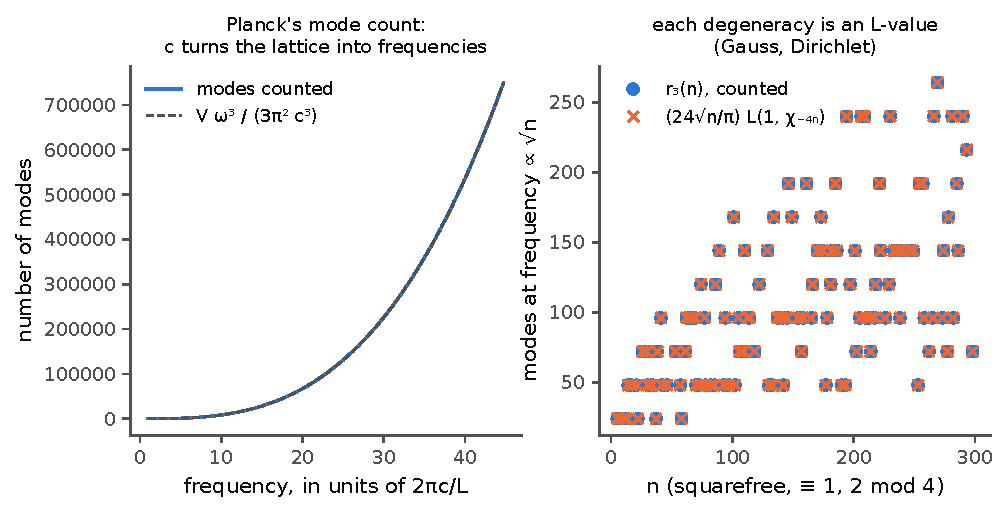
\includegraphics[width=0.92\textwidth]{light-modes}
  \caption{Left: modes of light in a periodic box, counted and from Planck's formula. Right: each multiplicity $r_3(n)$ against $(24\sqrt n/\pi)L(1,\chi_{-4n})$.}
  \label{fig:modes}
\end{figure}

\section{Gauss's forms are integer relativity in $2+1$ dimensions}

\begin{derivation}[the discriminant is a Minkowski form]\label{d:minkowski}
Write a binary form $ax^2+bxy+cy^2$ as the vector $(T,X,Y) = (a+c,\ b,\ a-c)$.
Then
\[
  b^2-4ac = X^2+Y^2-T^2,
\]
a Minkowski form of signature $(2,1)$.
The substitution $f(x,y)\mapsto f(\alpha x+\beta y,\gamma x+\delta y)$ by $\left(\begin{smallmatrix}\alpha&\beta\\\gamma&\delta\end{smallmatrix}\right)\in\SL(2,\Z)$ is linear in $(a,b,c)$ and preserves the discriminant.
So $\SL(2,\Z)$ acts on forms by integral Lorentz transformations ($\mathrm{PSL}(2,\R)\cong SO^+(2,1)$).
\end{derivation}

\begin{center}
\small
\begin{tabular}{@{}llll@{}}
\toprule
form & discriminant & vector & in the upper half-plane\\
\midrule
definite, e.g.\ $x^2+y^2$ & $<0$ & timelike: a massive particle & a point $\tau$ (its root)\\
degenerate, e.g.\ $x^2$ & $0$ & lightlike: a light ray & a cusp\\
indefinite, e.g.\ $x^2-xy-y^2$ & $>0$ & spacelike & a geodesic\\
\bottomrule
\end{tabular}
\end{center}

\noindent
The upper half-plane is the space of velocities.
A timelike vector $(T,X,Y)$ has velocity $(X/T,Y/T)$, of speed below $c=1$.
Rapidity, the relativistic measure of speed, is hyperbolic distance (Figure~\ref{fig:forms}).

\begin{derivation}[relative velocity]\label{d:velocity}
For definite forms $f,g$ of discriminants $D_f,D_g$, with $B(f,g) = b_fb_g - 2a_fc_g - 2a_gc_f$ the bilinear form of the discriminant, the relative rapidity $\eta$ satisfies $\cosh\eta = -B(f,g)/\sqrt{D_fD_g}$.
For $x^2+y^2$ and $x^2+xy+y^2$ this gives $\cosh\eta = 2/\sqrt3$, so $\tanh\eta = \tfrac12$.
\end{derivation}

\physical The Gaussian and Eisenstein forms, as particles, move relative to each other at exactly half the speed of light.
Equivalently, the hyperbolic distance from $i$ to $\rho$ is $\operatorname{artanh}\frac12 = 0.5493$.
The golden form $x^2-xy-y^2$ is spacelike; its geodesic is the shortest closed geodesic of note~05, which passes through $i$.

\begin{derivation}[class numbers count particles]\label{d:classes}
The class number $h(D)$ is the number of primitive integer particles on the mass shell $X^2+Y^2-T^2 = D$, up to integral Lorentz transformations.
The class number formula reads
\[
  h(D) = \frac{w_D\sqrt{|D|}}{2\pi}\,L(1,\chi_D).
\]
\end{derivation}

\noindent
The script checks the formula for all 122 fundamental discriminants $D>-400$.
\physical How many essentially different integer particles share a given mass is a Dirichlet $L$-value.

\begin{figure}[ht]
  \centering
  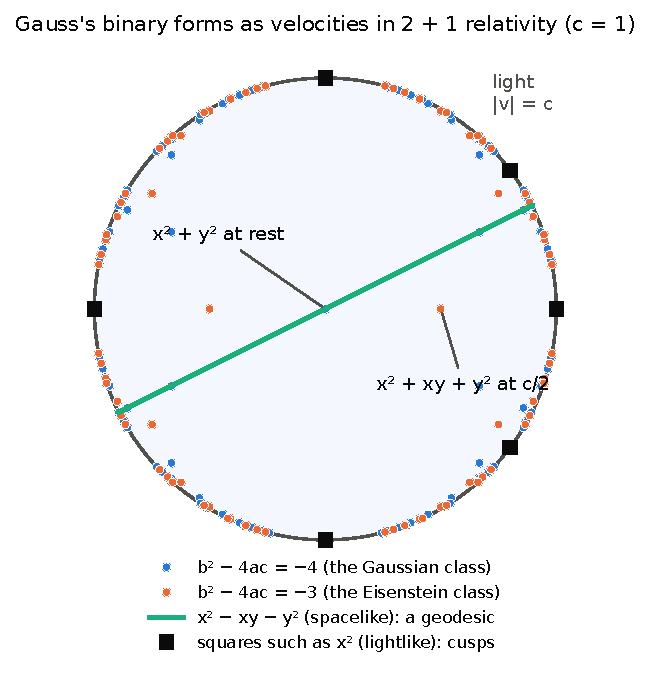
\includegraphics[width=0.62\textwidth]{light-forms}
  \caption{Binary forms as velocities with $c=1$ (the Klein disc). The forms of discriminant $-4$ and $-3$ accumulate towards light speed. The golden form is a chord (a geodesic), and squares such as $x^2$ sit on the light circle.}
  \label{fig:forms}
\end{figure}

\section{Spheres and mass shells}

Derivation~\ref{d:gauss} is a bridge.
The number of integer points on the sphere $x^2+y^2+z^2 = n$, in space, is 12 times the number of integer particles of mass $2\sqrt n$, in $2+1$ spacetime.
Both kinds of points spread evenly as they grow.
On the sphere this is Linnik's problem, solved by Duke; on the mass shell, they are the Heegner points on the modular surface \cite{Duke, Linnik}.
\physical On a sphere covered evenly, the heights are uniform on $[-1,1]$, which is Archimedes' hat-box theorem.
\begin{itemize}
\item The 7680 integer points on $x^2+y^2+z^2 = 1\,000\,005$ have heights uniform to a Kolmogorov--Smirnov distance of $0.0085$, and $7680 = 12\,h(-4\,000\,020)$.
\item The 11540 Heegner points with $20000\le|D|<20600$ put $0.639$ and $0.318$ of themselves above heights $1.5$ and $3$, where the hyperbolic areas predict $0.637$ and $0.318$ (Figure~\ref{fig:spheres}).
\end{itemize}

\begin{figure}[ht]
  \centering
  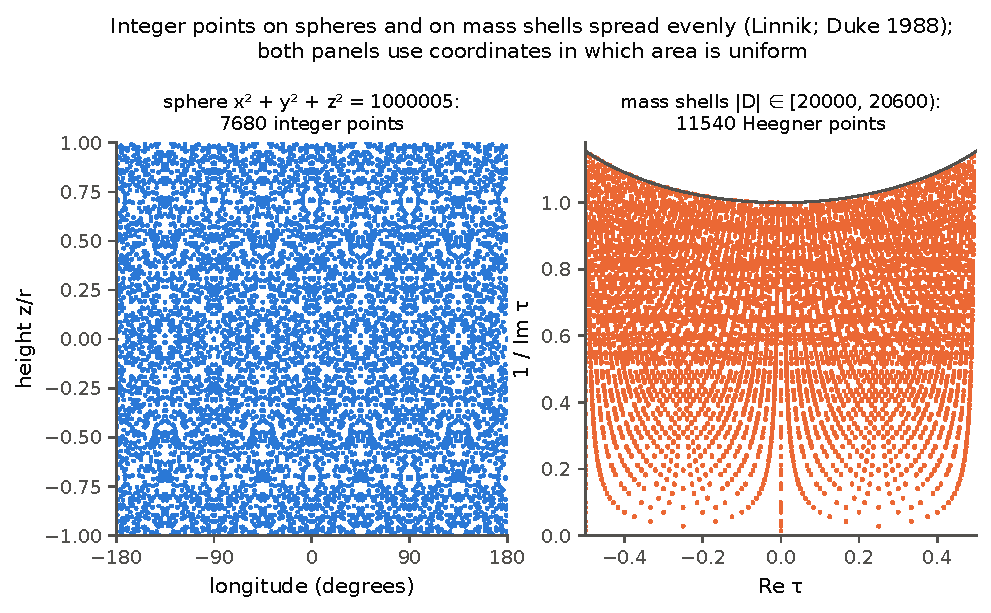
\includegraphics[width=0.92\textwidth]{light-spheres-shells}
  \caption{Left: integer points on a sphere, in (longitude, height), where area is uniform. Right: Heegner points in $(\mathrm{Re}\,\tau, 1/\mathrm{Im}\,\tau)$, where hyperbolic area is uniform.}
  \label{fig:spheres}
\end{figure}

\paragraph{Spheres and atoms.}
The harmonics of degree $l$ on the sphere form a space of dimension $2l+1$.
Summing over $l<n$ gives $n^2$, the degeneracy of the hydrogen level $n$ without spin.
The atom's degeneracy is the sphere's harmonics, counted.

\section{The $3+1$ light cone and the celestial sphere}

\begin{derivation}[Lorentz transformations are M\"obius maps]\label{d:mobius}
Write a spacetime point as a Hermitian matrix $X = \left(\begin{smallmatrix} t+z & x-iy\\ x+iy & t-z\end{smallmatrix}\right)$, so that $\det X = t^2-x^2-y^2-z^2$.
Each $A\in\SL(2,\C)$ acts by $X\mapsto AXA^*$, preserving $\det X$: a Lorentz transformation.
A light ray is $X = vv^*$ for a spinor $v\in\C^2$.
On the direction $\zeta = v_1/v_2$, a point of the celestial sphere $\C\cup\{\infty\}$, $A$ acts as the M\"obius map $\zeta\mapsto(a\zeta+b)/(c\zeta+d)$ \cite{PenroseRindler}.
\end{derivation}

\physical A Lorentz boost moves the stars on the sky by a M\"obius map.
The group $\SL(2,\Z[i])$ (Picard's group) preserves the Hermitian matrices with integer diagonal and Gaussian-integer off-diagonal entries.
So it is a lattice of Lorentz transformations built on the Gaussian integers.
The Bianchi groups $\mathrm{PSL}(2,\mathcal O_D)$ of the imaginary quadratic fields of note~02 act on hyperbolic 3-space, the velocity space of $3+1$ relativity, as $\SL(2,\Z)$ acts on the upper half-plane \cite{EGM}.
The script checks both statements on random matrices.

\section{The one pure number with $c$ in it}

The fine-structure constant $\alpha = e^2/(4\pi\varepsilon_0\hbar c)$ is dimensionless, so its value does not depend on units.
CODATA gives $1/\alpha = 137.035\,999\,084(21)$ \cite{CODATA}.
Eddington proposed $137$ exactly.
Wyler proposed $\frac{9}{8\pi^4}\big(\frac{\pi^5}{2^4\,5!}\big)^{1/4}$, from volumes of symmetric domains, which gives $137.036\,082$ \cite{Wyler}.
They miss by about 1.7 million and 4000 standard deviations respectively.
A derivation of a physical constant must survive this test, and none of the identities above attempts one.

\section{Speculation, and questions}

The author's working hypothesis, stated as a hypothesis, has three parts.
First, the speed of light is not a number to be derived but the slope that turns spacetime into a quadratic form.
Second, once space and time are counted in the same integers, the arithmetic of quadratic forms is the arithmetic of light.
Third, spherical phenomena belong to definite forms (spheres, $x^2+y^2+z^2$) and hyperbolic phenomena to indefinite ones (mass shells, light cones), and Gauss's theorem links the two.
\begin{question}
Is there a physical system in which an integral Lorentz group acts, so that class numbers appear as the degeneracies of its mass levels?
\end{question}
\begin{question}
Do the CM points of the Bianchi groups for $\Q(i)$ and $\Q(\sqrt{-3})$ have exact relative velocities, as $i$ and $\rho$ do ($c/2$), and do they organise the celestial sphere as the elliptic points organise the modular surface?
\end{question}

\section*{Status of the statements}

\begin{center}
\small
\begin{tabular}{@{}p{0.62\textwidth}l@{}}
\toprule
Statement & Grade\\
\midrule
$c$ exact by definition; unit conversions & \gradeConvention{} (SI), \gradeComputed\\
Derivations~\ref{d:planck}--\ref{d:mobius} & \gradeClassical\\
Mode counts; Gauss for $n\le3000$; $L$-value form; class number formula, $D>-400$ & \gradeComputed\\
Relative velocity $c/2$ of the Gaussian and Eisenstein forms & \gradeComputed\\
Even spreading on the sphere $n = 1\,000\,005$ and on mass shells & \gradeComputed; theorem \gradeClassical\\
Wyler and Eddington fail at CODATA precision & \gradeComputed\\
The hypothesis and Questions 1--2 & \gradeOpen\\
\bottomrule
\end{tabular}
\end{center}

\begin{thebibliography}{9}
\bibitem{SI} Bureau International des Poids et Mesures, \emph{The International System of Units (SI)}, 9th ed., 2019.
\bibitem{CODATA} E.~Tiesinga, P.~J. Mohr, D.~B. Newell and B.~N. Taylor, CODATA recommended values of the fundamental physical constants: 2018, \emph{Rev. Mod. Phys.} 93 (2021), 025010.
\bibitem{Duke} W.~Duke, Hyperbolic distribution problems and half-integral weight Maass forms, \emph{Invent. Math.} 92 (1988), 73--90.
\bibitem{EGM} J.~Elstrodt, F.~Grunewald and J.~Mennicke, \emph{Groups Acting on Hyperbolic Space}, Springer, 1998.
\bibitem{Grosswald} E.~Grosswald, \emph{Representations of Integers as Sums of Squares}, Springer, 1985.
\bibitem{Linnik} Yu.~V. Linnik, \emph{Ergodic Properties of Algebraic Fields}, Springer, 1968.
\bibitem{PenroseRindler} R.~Penrose and W.~Rindler, \emph{Spinors and Space-Time}, vol.~1, Cambridge University Press, 1984.
\bibitem{Wyler} E.~W. Weisstein, Wyler's constant, \emph{MathWorld}, \url{https://mathworld.wolfram.com/WylersConstant.html} (A.~Wyler, 1969).
\end{thebibliography}

\end{document}
